\documentclass[a4paper, 12pt]{article}
\usepackage[a4paper,top=2cm,bottom=2cm,left=1cm,right=1cm,marginparwidth=0.75cm]{geometry}

\usepackage[T2A]{fontenc}
\usepackage{mathtools}
\usepackage[utf8]{inputenc}
\usepackage[english, russian]{babel}
\usepackage{gensymb}
\usepackage{floatrow}
\usepackage{fancyhdr}


\usepackage{xcolor}

\pagecolor[rgb]{1,1,1} %black

\color[rgb]{0,0,0} %grey

\pagestyle{fancy}
\author{}
\title{Измерение вязкости воздуха по течению в тонких трубках}
\lhead{Работа 1.3.3}
\rhead{Севастьян Черняков Б05-207}
\date{}

\begin{document}
\selectlanguage{russian}
\maketitle
\textbf{Цель работы:} экспериментально исследовать свойства течения газов по тонким трубкам при различных числах Рейнольдса; выявить область применимости закона Пуазейля и с его помощью определить коэффициент вязкости воздуха.\hfill
\break
	
\textbf{В работе используются:} система подачи воздуха (компрессор, поводящие трубки); газовый счетчик барабанного типа; спиртовой микроманометр с регулируемым наклоном; набор трубок различного диаметра с выходами для подсоединения микроманометра; секундомер.


\section{Теоретическая часть}
Рассмотрим движение вязкой жидкости или газа по трубке круглого сечения. При малых скоростях потока движение оказывается ламинарным (слоистым), скорости частиц меняются по радиусу и направлены вдоль оси трубки. С увеличением скорости потока движение становится турбулентным, а слои перемешиваются. При турбулентном движении скорость в каждой точке быстро меняет величину и направление, сохраняется только средняя величина скорости.

Характер движения газа (или жидкости) в трубке определяется безразмерным числом Рейнольдса:
\[
	Re = \frac{vr\rho}{\eta}
\]
где $v$ -- скорость потока, $r$ -- радиус трубки, $\rho$ -- плотность движущейся среды, $\eta$ -- её вязкость. В гладких трубах круглого сечения переход от ламининарного движения к турбулентному происходит при $Re \approx 1000$.

При ламинарном течении объем газа $V$, протекающий за время $t$ по трубе длиной $l$, определяется формулой Пуазейля:
\begin{equation}
	Q = \frac{\pi r^4}{8 \Delta l \eta}(P_1 - P_2)
\end{equation}
В этой формуле $P_1 - P_2$ -- разность давлений в двух выбранных сечениях 1 и 2, расстояние между которыми равно $\Delta l$. Величину $Q$ обычно называют расходом. Формула (1) позволяет определять вязкость газа по его расходу.

Отметим условия, при которых справедлива формула (1). Прежде всего необходимо, чтобы с достаточным запасом выполнялось неравенство $Re < 1000$. Необходимо также, чтобы при течении не происходило существенного изменения удельного объёма газа (при выводе формулы удельный объём считался постоянным). Для жидкости это предположение выполняется практически всегда, а для газа --- лишь в тех случаях, когда перепад давлений вдоль трубки мал по сравнению с самим давлением. В нашем случае давление газа равно атмосферному ($10^3$ см вод. ст.), а перепад давлений составляет не более 10 см вод. ст., т. е. менее 1\% от атмосферного. Формула (1) выводится для участков трубки, на которых закон распределения скоростей газа по сечению не меняется при двидении вдоль потока.
\begin{figure}[H]
\center
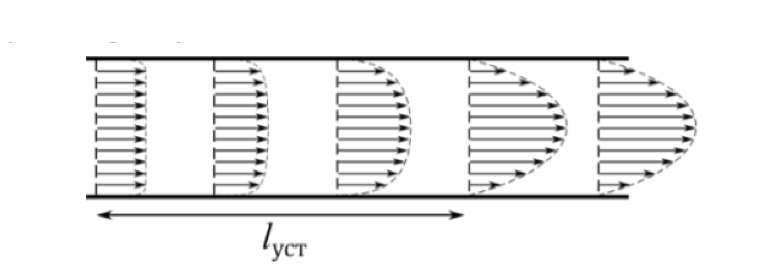
\includegraphics[scale=0.5]{potok.png}
\caption{Формирование потока газа в трубке круглого сечения}
\end{figure}
При втекании газа в трубку из большого резервуара скорости слоёв вначале постоянны по всему направлению. По мере продвижения газа по трубке картина распределения скоростей меняется, так как сила трения о стенку тормозит прилежащие к ней оси. Характерное для ламинарного течения параболическое распределение скоростей устанавливается на некотором расстоянии $a$ от входа в трубку, которое зависит от радиуса трубки $r$ и числа Рейнольдса по формуле 
\begin{equation}
	a \approx 0.2rRe
\end{equation}
Градиент давления на участке формирования потока оказывается больше, чем на участке с установившимся ламинарным течением, что позволяет разделить эти участки экспериментально. Формула (2) даёт возможность оценить дину участка формирования.

\section{Экспериментальная установка}

Схема экспериментальной установки изображена на Рис. \ref{233}. Поток воздуха
под давлением, немного превышающим атмосферное, поступает через газовый счётчик в тонкие металлические трубки. Воздух нагнетается компрессором, интенсивность его подачи регулируется краном К. Трубки снабжены
съёмными заглушками на концах и рядом миллиметровых отверстий, к которым можно подключать микроманометр. В рабочем состоянии открыта заглушка на одной (рабочей) трубке, микроманометр подключён к двум её выводам, а все остальные отверстия плотно закрыты пробками.

\begin{figure}[H]
    \centering
    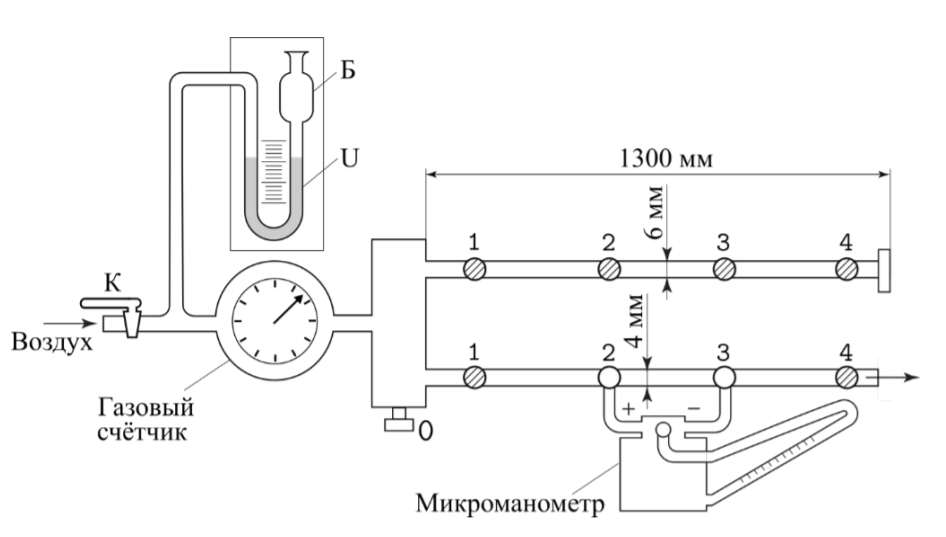
\includegraphics[scale=0.65]{expust.PNG}
    \caption{Экспериментальная установка}
    \label{233}
\end{figure}

Перед входом в газовый счётчик установлен водяной U-образный манометр. Он служит для измерения давления газа на входе, а также предохраняет
счётчик от выхода из строя. При превышении максимального избыточного
давления на входе счётчика ($\sim$ 30 см вод. ст.) вода выплёскивается из трубки
в защитный баллон Б, создавая шум и привлекая к себе внимание экспериментатора.


\textbf{Газовый счётчик.} В работе используется газовый счётчик барабанного
типа, позволяющий измерять объём газа $\Delta V$ прошедшего через систему. Измеряя время $\Delta t$ при помощи секундомера, можно вычислить средний объёмный расход газа $Q = \Delta V/ \Delta t$ (для получения массового расхода [кг/с] результат
необходимо домножить на плотность газа $\rho$).

\begin{figure}[H]
    \centering
    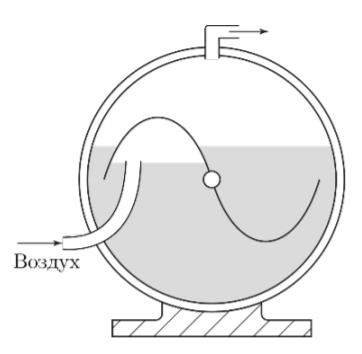
\includegraphics[scale=0.65]{gascounter.PNG}
    \caption{Газовый счетчик}
    \label{333}
\end{figure}


Работа счётчика основана на принципе вытеснения: на цилиндрической ёмкости жёстко
укреплены лёгкие чаши (см. Рис. \ref{333}, где для
упрощения изображены только две чаши), в которые поочередно поступает воздух из входной
трубки расходомера. Когда чаша наполняется,
она всплывает и её место занимает следующая
и т.д. Вращение оси предаётся на счётно-суммирующее устройство.
Для корректной работы счётчика он должен
быть заполнен водой и установлен горизонтально по уровню (подробнее см. техническое
описание установки).

\textbf{Микроманометр.} В работе используется жидкостный манометр с наклонной трубкой. Разность давлений на входах манометра измеряется по высоте
подъёма этилового спирта. Регулировка
наклона позволяет измерять давление в различных диапазонах.

На крышке прибора установлен трехходовой кран, имеющий два рабочих
положения — (0) и (+). В положении (0) производится установка мениска жидкости на ноль, что необходимо сделать перед началом работы (в процессе работы также рекомендуется периодически проверять положение нуля). В положении (+) производятся измерения.


\section{Обработка рузультатов измерений}

Эксперимент проводился при комнатной температуре $T_\text{комн}=297,4 K$, при атмофсерном давлении $P_\text{атм}=99,6 \pm 0.1$ кПа и при относительной влажности в помещении $\phi=83\%$.
При таких показателях окружающей среды теоретическое $Q_\text{кр} = 100 \pm 2 \text{мл/с}$ а $\Delta P_\text{кр} = 177 \pm 10\text{Па}$ для первой трубы и \\
$Q_\text{кр} = 137 \pm 3 \text{мл/с}$ а $\Delta P_\text{кр} = 64 \pm 5\text{Па}$

\begin{align}
    &Re_{\text{кр}} = \frac{\mu P Q}{\pi r R T \eta} = 1000 \quad \text{отсюда следует} \quad Q_{\text{кр}} = \frac{Re \pi r R T \eta}{\mu P}  \\
    &\sigma_{Q_{\text{кр}}} = Q_{\text{кр}} \cdot \sqrt{(\frac{\sigma_r}{r})^2 + (\frac{\sigma_T}{T})^2 + (\frac{\sigma_P}{P})^2} \\
    &\Delta P_{\text{кр}} =\frac{ 8Q_{\text{кр}} L \eta}{\pi r^4}  \quad \sigma_{\Delta P_{\text{кр}}} = \Delta P_{\text{кр}} \cdot \sqrt{(\frac{\sigma_Q}{Q})^2 + (\frac{\sigma_L}{L})^2 +  16 (\frac{\sigma_r}{r})^2}
\end{align}

По формуле (2) формирование распределения скоростей происходит на расстоянии ~39см.

Давление, измеряемое микроманометром, определяется по формуле:
\[
P=9,81 \cdot K \cdot h 
\]
где $h$ -- показание макроманометра, $K$ -- коэффициент наклона, $P$ -- Давление в паскалях.

\subsection{Зависимость разности давлений от расхода}
Эксперимент проводился на первой трубе с диаметром $d_1=3,95\ \pm\ 0,05$ мм. Данные изменрений приведены в табилце 1.

\floatsetup[table]{capposition=top}
\begin{table}[H]
    \centering
    \begin{tabular}{|c|c|c|c|c|}
        \hline $h$, мм & $\Delta V$, л & $\Delta t$, с & $\Delta P$, Па & $Q$, мл$/$с \\
        13 & 3 & 220 & 25.506 & 13.6 \\ \hline
        20 & 3 & 135 & 39.24 & 22.2 \\ \hline
        27 & 3 & 98 & 52.974 & 30.6 \\ \hline
        33 & 3 & 64 & 64.746 & 36.9 \\ \hline
        40 & 4 & 86 & 78.48 & 46.5 \\ \hline
        50 & 4 & 69 & 98.1 & 58.0 \\ \hline
        56 & 4 & 60 & 109.872 & 66.7 \\ \hline
        65 & 4 & 53 & 127.53 & 75.5 \\ \hline
        72 & 5 & 61 & 141.264 & 82.0 \\ \hline
        80 & 5 & 55 & 156.96 & 90.9 \\ \hline
        89 & 5 & 51 & 174.618 & 98.0 \\ \hline
        96 & 5 & 50 & 188.352 & 100.0 \\ \hline
        102 & 6 & 48 & 200.124 & 125.0 \\ \hline
        110 & 7 & 46 & 215.82 & 152.2 \\ \hline
        125 & 8 & 45 & 245.25 & 177.8 \\ \hline
        165 & 9 & 41 & 323.73 & 219.5 \\ \hline
        195 & 10 & 39 & 382.59 & 256.4 \\ \hline
        240 & 11 & 35 & 470.88 & 314.3 \\ \hline
    \end{tabular}
    \caption{Результаты измерений разности давлений от расхода}
    \label{tab:q(p)}
\end{table}

По результатам измерений был построен график 1. По угловому коэффициенту и формуле (1) можно оценить вязкость воздуха. Она составила $\eta = 1,87 \pm 0,09 \times 10^{-5}$ Па$\cdot$с.

\begin{figure}[H]
    \centering
    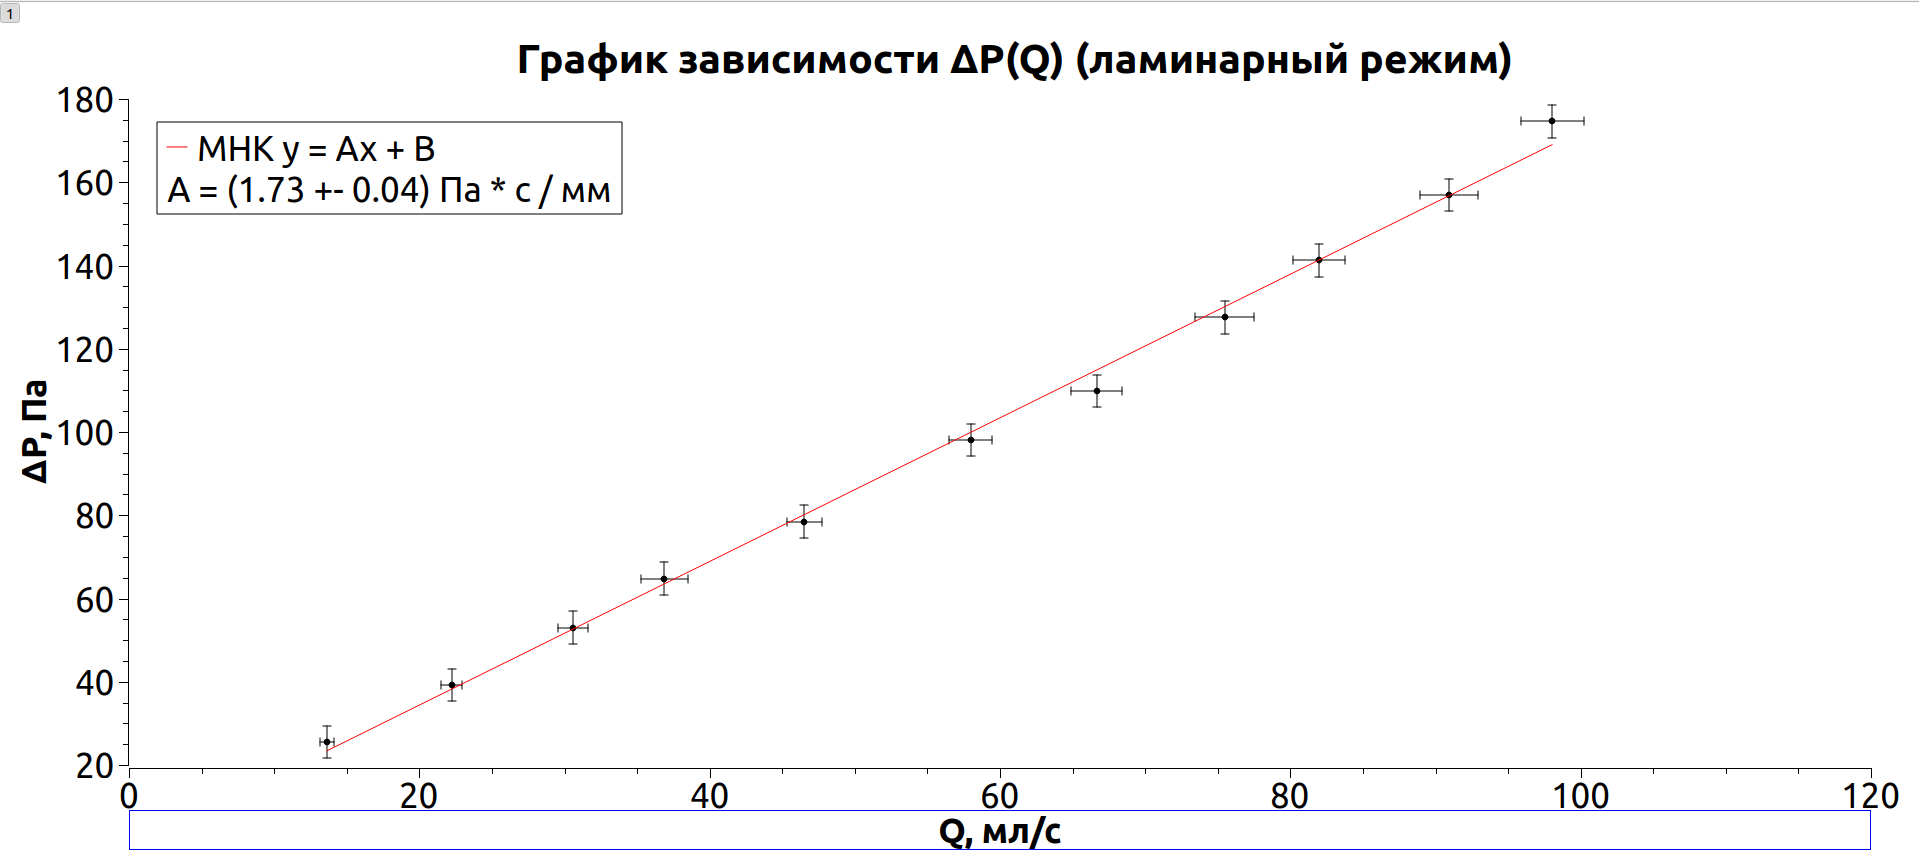
\includegraphics[scale=0.25]{chart.png}
    \label{p(q)}
\end{figure}


\begin{figure}[H]
    \centering
    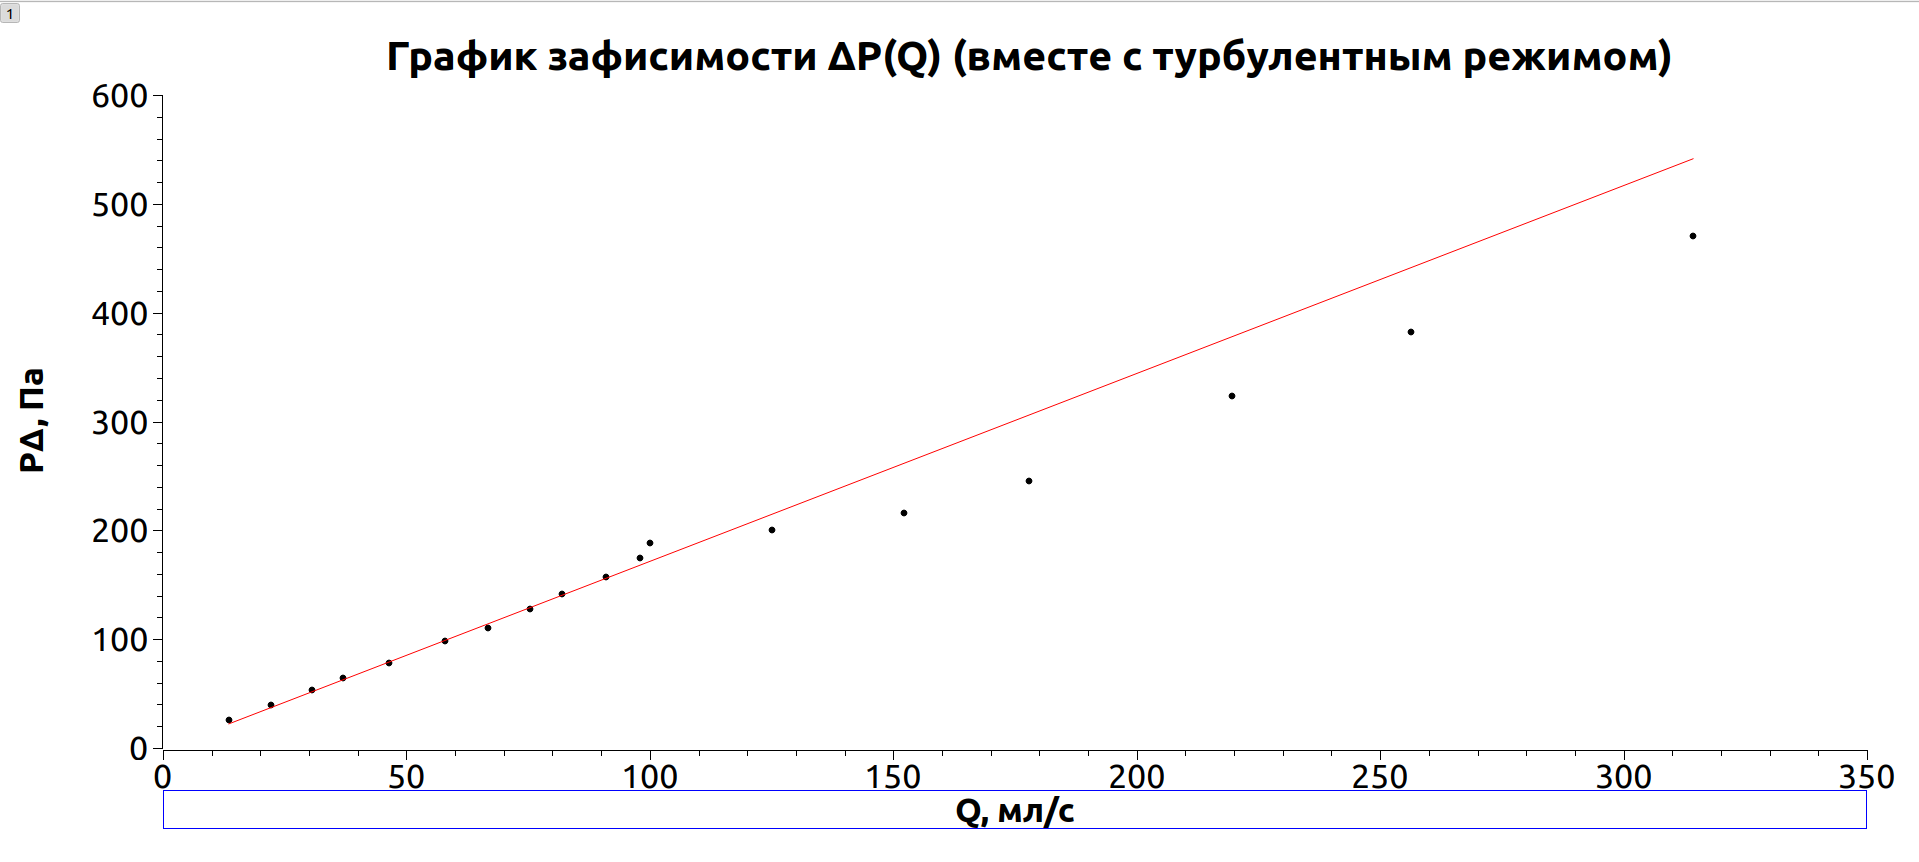
\includegraphics[scale=0.25]{2.png}
    \label{p(q)}
\end{figure}

По графику видно, что переход к турбулентному режиму происходит при $\Delta P = 174 \pm 10 \text{Па и при} Q = 98 \pm 2 \text{мл/с} $ что совпадает с теоретически посчитанными значениями. Число Рейнольдса в этой точке равно $Re = 996 \pm 8$ 


\begin{align}
    &Re = \frac{Q P \mu}{\pi R T r \eta} \quad \sigma_{Re} = Re \cdot \sqrt{(\frac{\sigma_{Q}}{Q})^2 + (\frac{\sigma_{P}}{P})^2 + (\frac{\sigma_{T}}{T})^2 + (\frac{\sigma_{r}}{r})^2 + (\frac{\sigma_{\eta}}{\eta})^2}
\end{align}

погрешности измеряемых величин:
\centering
\newline

\begin{align}
    &\sigma_{h} = 2 \text{мм} \quad \sigma_{V} = 0.1 \text{л} \\
    & \sigma_{P} = (9.81 * \sigma_{h} * 0.2) \text{Па} = 3.924 \text{Па}
    &\sigma_Q^\text{сист} = Q \cdot \varepsilon_{Q} = Q \cdot \sqrt{(\frac{\sigma_{T}}{T})^2 + (\frac{\sigma_{V}}{V})^2} 
\end{align}


Угловой коэффициент измерялся по МНК: 
\begin{align}
    & A = \frac{\langle Q \Delta P \rangle}{\langle Q^2 \rangle} &
    & \sigma_A^\text{случ} = \frac{1}{\sqrt{n}}\cdot \sqrt{\frac{\langle \Delta P \rangle ^ 2}{\langle Q \rangle ^ 2} - A^2} \\
    & \sigma_A^\text{сист} = A \cdot \sqrt{\epsilon_{\Delta P}^2 + \epsilon_{Q}^2}
    && \sigma_A^\text{полн} = \sqrt{(\sigma_A^\text{сист})^2 + (\sigma_A^\text{случ})^2}
\end{align}




из формулы (1) величина 
\begin{align}
    \eta = \frac{\pi r^4}{8 L} \cdot A и &&
    && \sigma_{\eta} = \eta \cdot \sqrt{16 (\frac{\sigma_r}{r})^2 + (\frac{\sigma_L}{L})^2 + (\frac{\sigma_A}{A})^2}
\end{align}

аналогичные измерения для трубки с диаметром $d_1=5,10\ \pm\ 0,05$ мм. Данные изменрений приведены в табилце 2.





\floatsetup[table]{capposition=top}
\begin{table}[H]
    \centering
    \begin{tabular}{|c|c|c|c|c|}
        \hline $h$, мм & $\Delta V$, л & $\Delta t$, с & $\Delta P$, Па & $Q$, мл$/$с \\
        \hline 11 & 3 & 88.3 & 21.5 & 33.9 \\ \hline
        30 & 5 & 43.8 & 58.9 & 114.1 \\ \hline
        20 & 5 & 70.3 & 39.2 & 71.1 \\ \hline
        40 & 5 & 36.9 & 78.5 & 135.5 \\ \hline
        50 & 5 & 32.3 & 98.1 & 154.8 \\ \hline
        65 & 5 & 30.7 & 127.5 & 162.8 \\ \hline
        76 & 5 & 28.1 & 149.1 & 177.9 \\ \hline
        80 & 5 & 27.5 & 156.9 & 181.8 \\ \hline
        90 & 5 & 25.6 & 176.5 & 195.3 \\ \hline
    \end{tabular}
    \caption{Результаты измерений разности давлений от расхода}
    \label{tab:q(p)}
\end{table}
По результатам измерений был построен график. По угловому коэффициенту и формуле (1) можно оценить вязкость воздуха. Она составила $\eta = 1,77 \pm 0,09 \times 10^{-5}$ Па$\cdot$с, таким образом, величина, измеренная на второй трубке совпала с измеренной на первой трубке величиной. Из-за меньшего количества измерений сложно четко определть точку перехода к турбулентному режиму, но по графику видно, что зависимость соответствует теоретическому значению \\ 
(точка Q = 137 мл/с и $\Delta P$ = 64 Па лежит на участке перехода к турбулентниму режиму) 
\begin{figure}[H]
    \centering
    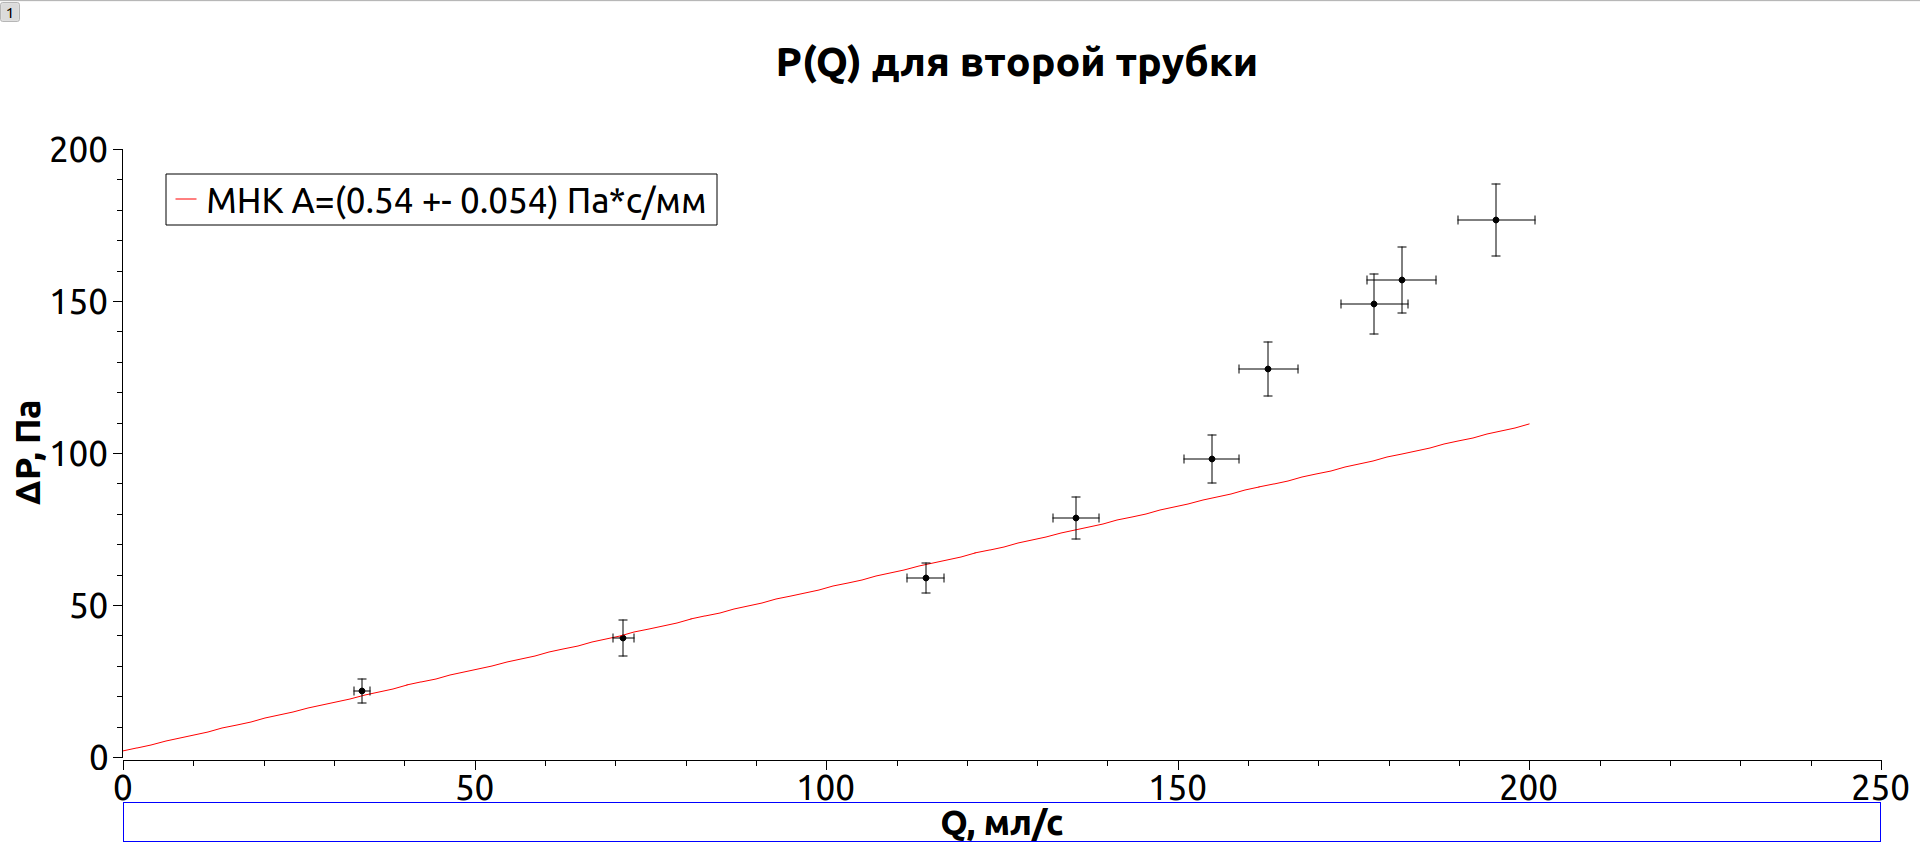
\includegraphics[scale=0.25]{chart2.png}
    \label{p(q)}
\end{figure}


\subsection{Зависимость разности давлений от длины участка}

Здесь измерения проводились на трубах 1 и 2 с диаметрами $d_1 = 3,95 \pm 0,05$ мм и $d_2 = 5,10 \pm 0,05$ мм, с расходами $Q_1 \approx 89,0$ мм/с и $Q_2 \approx 107,8$ мл/с соответственно.
Результаты измерений приведены в таблице \ref{p1}.

\begin{table}[H]
    \centering
    \begin{tabular}{|c|c|}
        \hline \multicolumn{2}{|c|}{$Q=89,0$ мл/с, $d=3,95$ мм} \\ \hline
        $x$, см & $\Delta P$, Па \\ \hline
        10,9 &  82,3 \\ \hline
        40,9 &  186,2 \\ \hline
        80,9 &  313,6 \\ \hline
        130,9 & 450,8 \\ \hline
        \multicolumn{2}{c}{} \\
        \hline \multicolumn{2}{|c|}{$Q=107,8$ мл/с, $d=5,10$ мм} \\ \hline
        10,9 &  123,6 \\ \hline
        40,9 &  229,6 \\ \hline
        80,9 &  323,7 \\ \hline
        130,9 & 455,2 \\ \hline
    \end{tabular}
    \caption{Зависимость давления от длины}
    \label{p1}

\end{table}

\begin{figure}[H]
    \centering
    \label{}
    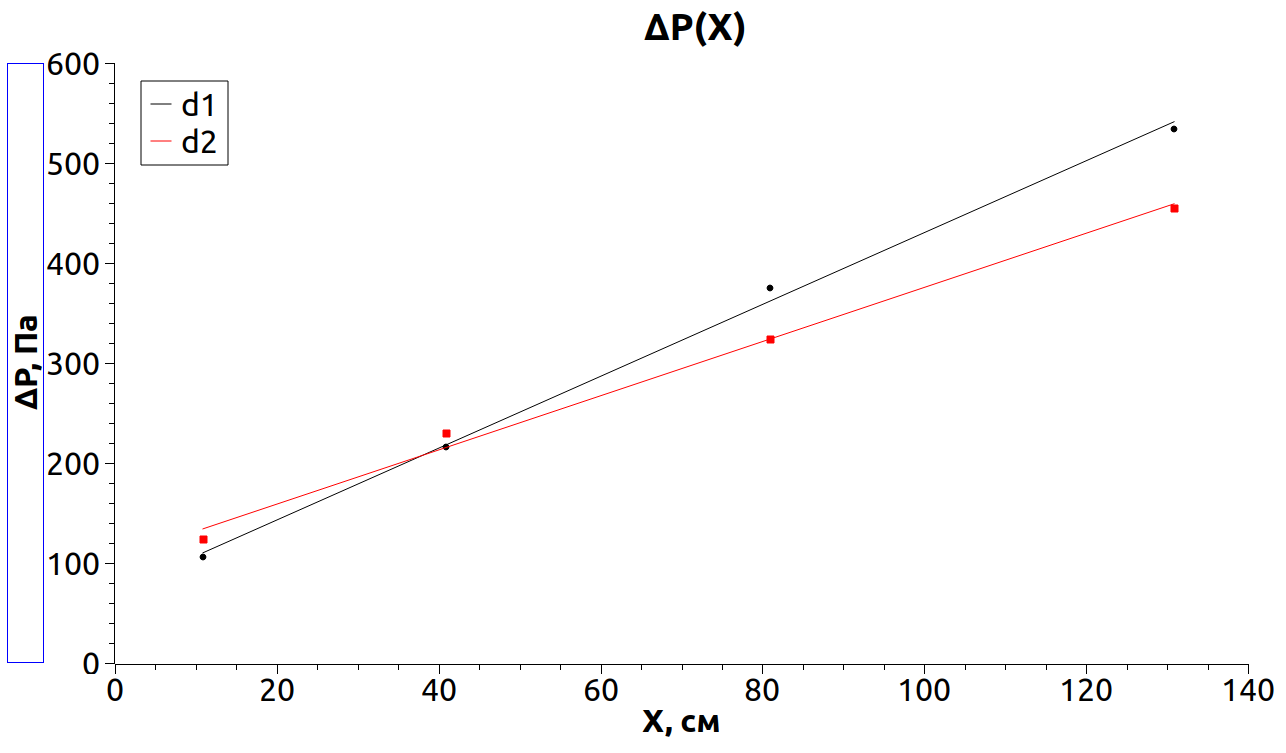
\includegraphics[scale=0.40]{p(x).png}
    \caption{Зависимость разности давлений от длины}
\end{figure}


\section{Выыод} 
Экспериментально исследовались свойства течения газов по тонким трубкам; найдены критические значения расхода, давления и число Рейнольдса для перехода в турбулентный режим, значения совпали с экспериментальными. Также
	определен коэффициент вязкости воздуха.
	\begin{align}
		\eta_1 = (1.87\pm 0.09)\text{ Па}\cdot\text{с} \quad \text{и} \quad \eta_2 = (1.77\pm 0.09)\text{ Па}\cdot\text{с}
	\end{align}
	
\end{document}